\documentclass{../resources/sig-alternate-05-2015}

\usepackage{todonotes}
\usepackage{fontspec}
\usepackage{makeidx}
\usepackage{rotating}
\usepackage{booktabs}
\usepackage{multirow}
\usepackage{svg}
\usepackage[scientific-notation=true]{siunitx}
\usepackage[
backend=biber,
style=numeric,
sorting=none,
doi=false,isbn=false,url=false
]{biblatex}
\addbibresource{../resources/lib.bib}

\setmonofont{DejaVu Sans Mono} 
\pagenumbering{arabic}

\makeatletter
\def\@copyrightspace{\relax}
\makeatother

\begin{document}

\title{Generating meaningful video thumbnails to improve user experience in video applications}
\subtitle{Master Thesis Information Studies}

\author{
Jorick van Hees \\
\texttt{\textbf{Blue Billywig}}\titlenote{Blue Billywig, Catharina van Renneslaan 20, 1217 CX Hilversum, The Netherlands} \\
\texttt{\textbf{University of Amsterdam}} \\
\texttt{Graduate School of Informatics} \\
\texttt{jorick.vanhees@student.uva.nl}
}

\maketitle

\abstract{We present a novel way to provide a visual preview of a video in the form of video thumbnails. This video thumbnail is an alternative to the static image thumbnail, which is much used in todays interfaces and are often the only visual clue for the user to get a sense of the contents of the video. The video thumbnail is designed to improve the user experience of video navigation structures. We present a method that automatically generates these video thumbnails in an ambiguous domain using clustering techniques on concept features, metadata analysis to generate topics, and a comparison to manually selected static thumbnails in order to evaluate the results. The resulting video thumbnails are tested against static thumbnails in a user study where we measure information and engagement in user experience. Based on the significant improvement that we found regarding information, we consider video summarisation techniques to provide a solid groundwork when generating video thumbnails. The characteristic intent of the video thumbnail emphasises the need for alterations to these techniques in order to improve engagement towards the audience.}


\printccsdesc

\category{I.2.10}{Vision and Scene Understanding}{Video analysis}
\category{H.5.2}{User Interfaces}{Graphical user interfaces (GUI)}

\keywords{Video thumbnail generation, Interfaces}

\section{Introduction}
\label{introduction}
% Method, approach, (framework), pipeline

% Intro:
% Placement of the work in community
% What propose?
% Brief reflection
% Research question

% Thumbnail
Thumbnail images for videos are used all over the web. They are static representations for videos, and provide a visual preview of the video itself. In combination with a title and description, they form one of the most common interfaces when dealing with a collection of videos. They increase the accuracy when conducting searches in video databases, improve the aesthetics of an overview page, and can increase engagement when appealing thumbnails are used.

% Video thumbnail
The video thumbnail is a preview of the full video in the form of a five-second excerpt containing no audio, which conveys the contents of the video in a more expressive manner. In this work, we describe a method that automatically generates these video thumbnails using state-of-the-art techniques like concept feature extraction and topic-dependent metadata analysis. With the addition of static thumbnails selected by experts as training data, we provide a novel way of conveying the purposes of the static thumbnail to the video thumbnail. This way, our approach has the ability to adjust to the specific requirements in engagement and information regarding the end-user, providing drop-in replacements for existing thumbnails.

With the generated video thumbnails, we analyse the effect on user experience and discuss the use of video summarisation techniques in the automatic video thumbnail generation. We hypothesise that the use of a video thumbnail instead of a static thumbnail will improve the user experience on two fronts. The user is more engaged to watch the full video, and will be more informed about the contents of the video. Furthermore, we hypothesise that video summarisation techniques will provide solid ground to generate a thumbnail, but require adjustments to better suit the intent of a video thumbnail. In order to test these hypothesis, two research questions are formulated:

\begin{itemize}
	\item How can we build a system that automatically generates video thumbnails that have a positive effect on the user?
	\item How do video thumbnails created by the system affect users regarding engagement and information?
\end{itemize}

% What did we do with this
Using a real world dataset in an ambiguous domain, the video thumbnail results of our method are challenged in a user survey against their static counterparts, where we test video previews with and without a thumbnail. These video previews are tested on information and engagement towards the user.

% What are the results and why are they awesome
The user study highlights the fact that the video thumbnail can match the performance of a static thumbnail without any problems. In addition, the results also point out that our approach of using a static thumbnails as training data is very effective in conveying the essence of the video, compared to a manually selected static thumbnail by a professional news editor. Finally, we conclude that our findings pose interesting opportunities in interface design and video analysis.

\subsection{Basic concepts \& related work}

\label{related work}

Work in the field of video summarisation has a lot of common ground with the generation of video thumbnails. Both use similar data to extract the desired information from a video and its metadata, the same techniques in computer vision is used to process the data and the end result could be very similar. 

One could argue that the results from video summarisation could be used in some implementations of the video thumbnails. However, the use cases in both domains are different in terms of user engagement. In general, a summary tries to accurately describe the contents of the video, which eliminates the need to view the full video. The goal of the thumbnail is to engage the user to view the full video, it tries to show just enough to trigger the user to view the remaining content. Since the implementation scenario and intention of the video thumbnail are different from video summaries, the methods used to generate video summarisation require alterations to meet the specific demands of the video thumbnail.

\paragraph{User engagement}
\label{section: user engagement}

User engagement in relation to (web) applications is the quality of experience and interaction of the user with an application. We can describe user engagement as time, attention and emotion that users put into the application \cite{Lehmann:2012ia}, but the whole concept of user engagement is far more complex than these aspects. In an extensive study towards the concept of engagement in various fields of work by \textcite{OBrien:2008km}, four stages of engagement are described, along with the attributes that are crucial in each stage.

% point of engagement, period of sustained engagement, disengagement, and reengagement
The video thumbnail is mainly an aesthetic element in the application of videos and their previews. As described in \textcite{OBrien:2008km}, aesthetics are crucial in the point of engagement, disengagement and the period of sustained engagement. Video previews can be viewed as a primary factor in the state `point of engagement', where the video itself is a factor in the `period of sustained engagement'. The study lists four attributes that present opportunities for the engagement of users in these stages: Aesthetic elements are pleasing or attention getting, Novel presentation of information, Interest, and becoming situated in the “story” of the application.

The novelty of the video thumbnail could play an important role in the engagement of users, static thumbnails are a common feature in todays interfaces and video thumbnails are a new way of presenting the information. The aesthetic of the video thumbnail very much depends on the method of creating a video thumbnails. The inclusion of moving images in the preview could be important with regards to the attention. Finally, the interest of the user and the `story' of the application could be enhanced by selecting the right shots from the video to use in the preview.

\paragraph{Event detection}
Existing methods for video event detection based on the TRECVID Media Event Detection Task \cite{1178722} often use the provided training data. In our approach, no training data is available for our specific goal of video thumbnails. However, we can use a number of techniques in order to extract the most characteristic frames from the video. Clustering frame vectors is a technique that is used in order to find related parts in the video. Concept features are extracted from frames with a standard frame interval, which are then clustered using unsupervised algorithms like K-means or a hierarchical variant of K-means. These clusters can be used in video summarisations to show a variety of video contents \cite{Mettes:2015vg,Ajmal:2012hi}.

\paragraph{Video navigation}
\label{section: video navigation}
There are a lot of interfaces designed to assist humans in navigating a video library. A summary by \textcite{Schoeffmann:2010iw} describes over 40 different interfaces that use different techniques to allow convenient browsing through a collection of videos. These range from displaying a key frame best describing the video, or a collection of keyframes with their sizes related to the importance of the frame. Most of these interfaces feature a system that automatically determines what to display on the screen, taken into consideration the different conditions in which the system is used. A study by \textcite{Hurst:2011jx} describes a user study to the recognition of video using different thumbnail sizes, numbers and various movement in the thumbnails. The study shows that users are able to handle multiple small thumbnails on mobile devices, especially when the thumbnails included motion. Since one of the goals of the video thumbnail is to improve the navigation of users in a news media website, video navigation literature could especially prove useful in the design and implementation of video thumbnails in overview pages.

\paragraph{Static thumbnail generation}
\label{section: static thumbnails}
The issue of video navigation using thumbnails has been an active topic of research. A \citeyear{Kim:2015co} study by \textcite{Kim:2015co} describes a method of automatically combining video frames to generate a thumbnail containing more information that a single frame. Another study describes thumbnail candidate selection using image quality evaluation \cite{Zhang:2014jg}. A combination of internal and external analysis of the video content to select thumbnails is used by a study by \textcite{Liu:2015ux}. The techniques and analysation methods that are featured in these methods can possibly be of use when evaluating the generated video thumbnails.

Many approaches to generating thumbnails use a ranking of different frames to propose a suitable thumbnail \cite{Choi:2015gm,Zhang:2012eo,Gao:2009dx}. In static thumbnail generation, this ranking can be used to select the best thumbnail. In video thumbnail generation (or other video navigation interfaces) the ranking can be used to create a composition of the video. This creates opportunities to generate video thumbnails that consist of different shots from the original video.


\section{Generating video thumbnails}
\label{section: system description}
The main body of this paper consists of the design of a method that is able to generate video thumbnails based on textual metadata and the video itself, trained on static thumbnails selected by experts. We set a number of requirements for our method:

\begin{itemize}
	\item The generated thumbnail only contains a single video segment extracted from the video, not a compilation of video segments.
	\item Contents of the video thumbnail should be appropriate for the intention of a thumbnail.
	\item Our method should suited for the generation of video thumbnails in an ambiguous domain.
\end{itemize}

The approach can be divided into five major stages: Feature extraction, candidate selection, candidate evaluation and topic-based model training. In the first stage, a number of moments in the video are selected and labeled as candidates. In the second stage, candidates are labeled with a positive or negative value based on their similarity to a thumbnail selected by an expert (referred to as the `selected thumbnail'). In the third stage, all videos in the dataset are clustered based on topics derived from their metadata. In the fourth and final stage, an SVM is trained for each cluster using the labeled candidates from each video in that cluster.

\subsection{Dataset requirements}
\label{section: dataset requirements}
In order to generate a meaningful video thumbnail, training examples in the form of static thumbnails are required in the dataset to train models that can evaluate and rank video thumbnail candidates. We use human-selected images that are used as a thumbnail for each video, since they contain the concepts that represent the video best from a human perspective. Another advantage of using the static thumbnail as evaluation data, is that it has the same purpose as the video thumbnail that our method creates. Since our approach should be suitable for all sorts of news videos, the dataset is not limited to a single domain. The required size of the dataset should be around the hundreds of videos, based on earlier research in video summarisation \cite{Almeida:2012be,Christel:2004in,Money:2008fn} and the fact that we are clustering our samples based on topics (section \ref{topic clustering}).

\subsection{Feature extraction}
\label{section: feature extraction}
Features from the video are extracted from individual frames with 1 frame per second using a convolutional neural network, trained on the ImageNet dataset \cite{Krizhevsky:2012wl} using Caffe \cite{Jia:2014cm}. The result is a high-level sparse feature representation of the frame with 1000 dimensions, which is used throughout the system as a representation of the frame. This technique of extracting features proves to be very effective for event-detection \cite{Habibian:2013ks,Althoff:2012gf,Jiang:2012fy} and video summarisation \cite{Ajmal:2012hi,Mazloom:2015el}.

\subsection{Candidate selection}
\label{section: candidate selection}

Instead of evaluating all possible frames in a video using a sliding window, a number of candidates are selected from the video. The selection algorithm is inspired by the bag-of-fragments as described in \cite{Mettes:2015vg}. Work in video summarisation and event detection use similar clustering techniques in order to establish a semantic structure in the video \cite{Yuan:2011fu,Habibian:2014dc}. This semantic structure can be utilised to discover the most representing window for every cluster, which can be used as candidates. A schematic overview of this method is shown in figure \ref{figure: candidate selection scheme}.

A comprehensive list of video thumbnail candidates is generated using a sliding window of 5 seconds with 1 fps. The video frames in the window are max-pooled into a vector representation that represents every concept in the video thumbnail. In order to prune the list of candidates, the video thumbnail is compared to a bag-of-fragments representation of the full video. The bags of fragments are created with the features extracted from all frames, clustered using K-means. The number K is calculated using the length of the video $K = \frac{frames}{20 * fps}$. The similarity between the video thumbnail and each BoF is measured using cosine similarity. The resulting similarity vector (with K dimensions) is then normalised, to prioritise the most representing video thumbnail for each BoF. Finally, a ranking is made for each BoF where the top result in each ranking is selected as thumbnail candidate. A visualisation of this method applied to a video can be found in figure \ref{figure: topic clustering example}.

\begin{figure}[h]
	\centering
	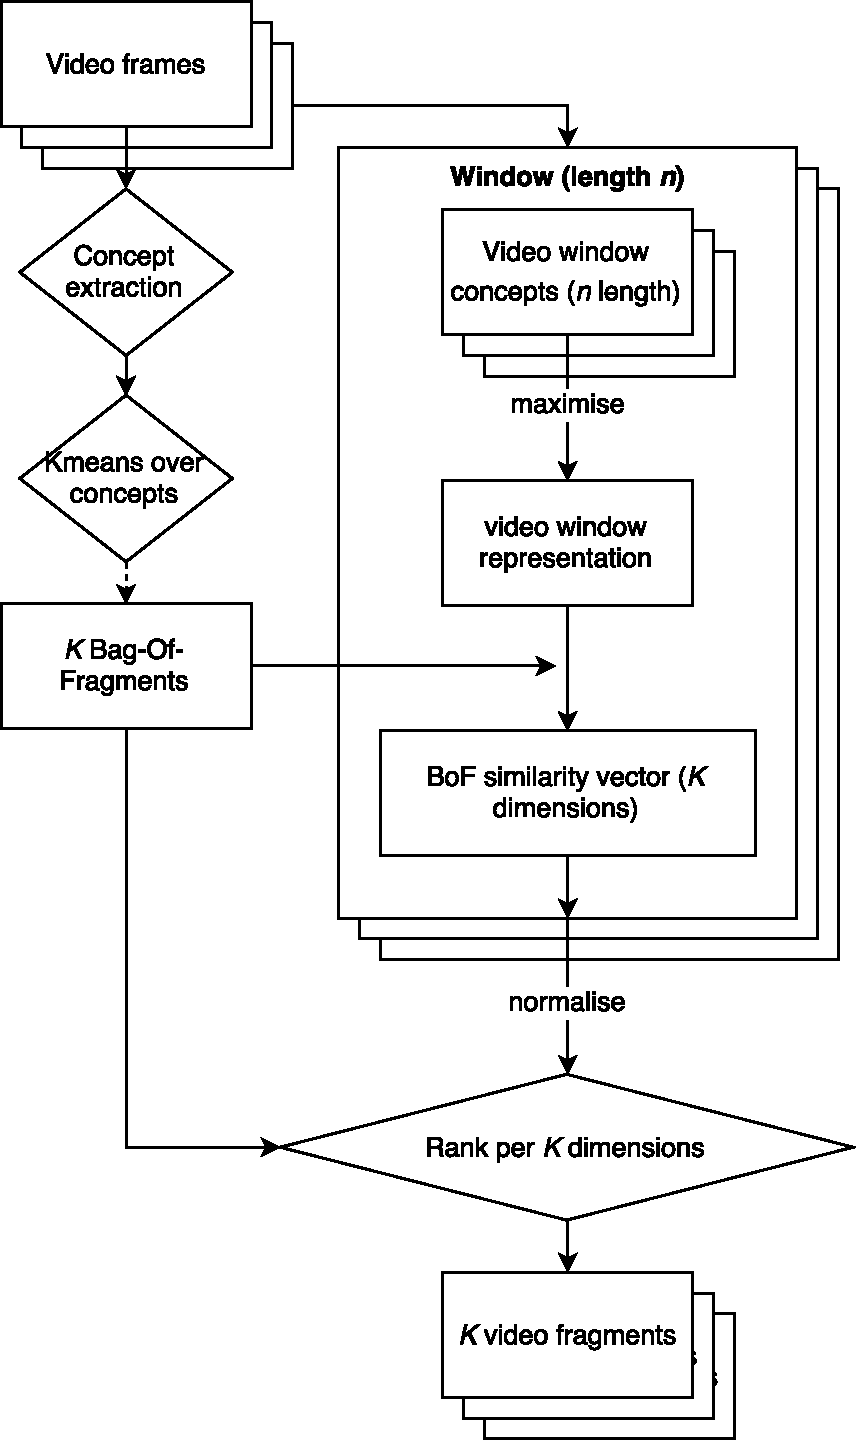
\includegraphics[width=0.8\linewidth]{resources/candidate-selection}
	\caption{A schematic overview of the candidate selection.}
	\label{figure: candidate selection scheme}
\end{figure}

\subsection{Candidate evaluation}
\label{section: candidate evaluation}

The resulting list of candidates is ranked based on the human-selected static thumbnail for that specific video. The same method of extracting features from the video is used on the static thumbnail, which results in a concept vector that can be compared to concept vectors extracted from the video frames. For every candidate, the cosine similarity between the candidate vector representation (as described in section \ref{section: candidate selection}) and the thumbnail concept vector is calculated. A schematic overview of this process is shown in figure \ref{figure: candidate evaluation scheme}.

\begin{figure}[h]
  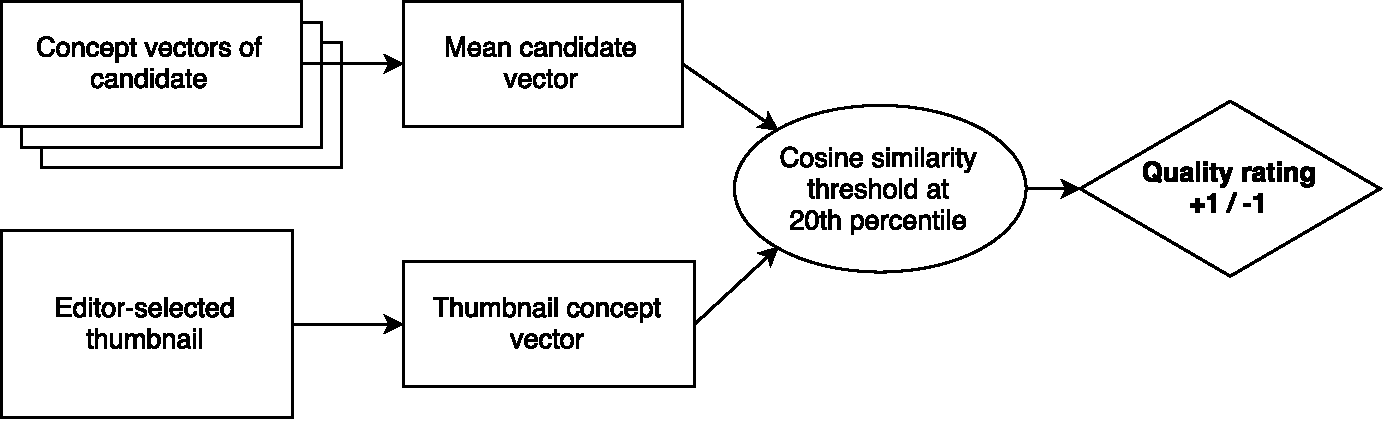
\includegraphics[width=\linewidth]{resources/candidate-evaluation}
  \caption{Evaluation the generated candidates using thumbnails selected by an editor.}
  \label{figure: candidate evaluation scheme}
\end{figure}

Since the resulting similarity values are very diverse across the dataset, a top $N$ percentile selection is used to determine positive ($+1$) and negative ($-1$) values which can later be used to train the SVM models. As shown in figure \ref{figure: thumbnail similarity}, the similarity values between candidates and the thumbnail are highly irregular across different videos. A threshold based on a percentile is therefor more suited to create a balanced training set that includes data from all videos. The $N$ value is selected at 20, since it provides a balanced distribution of positive and negative examples used as training data.

\begin{figure}[h]
  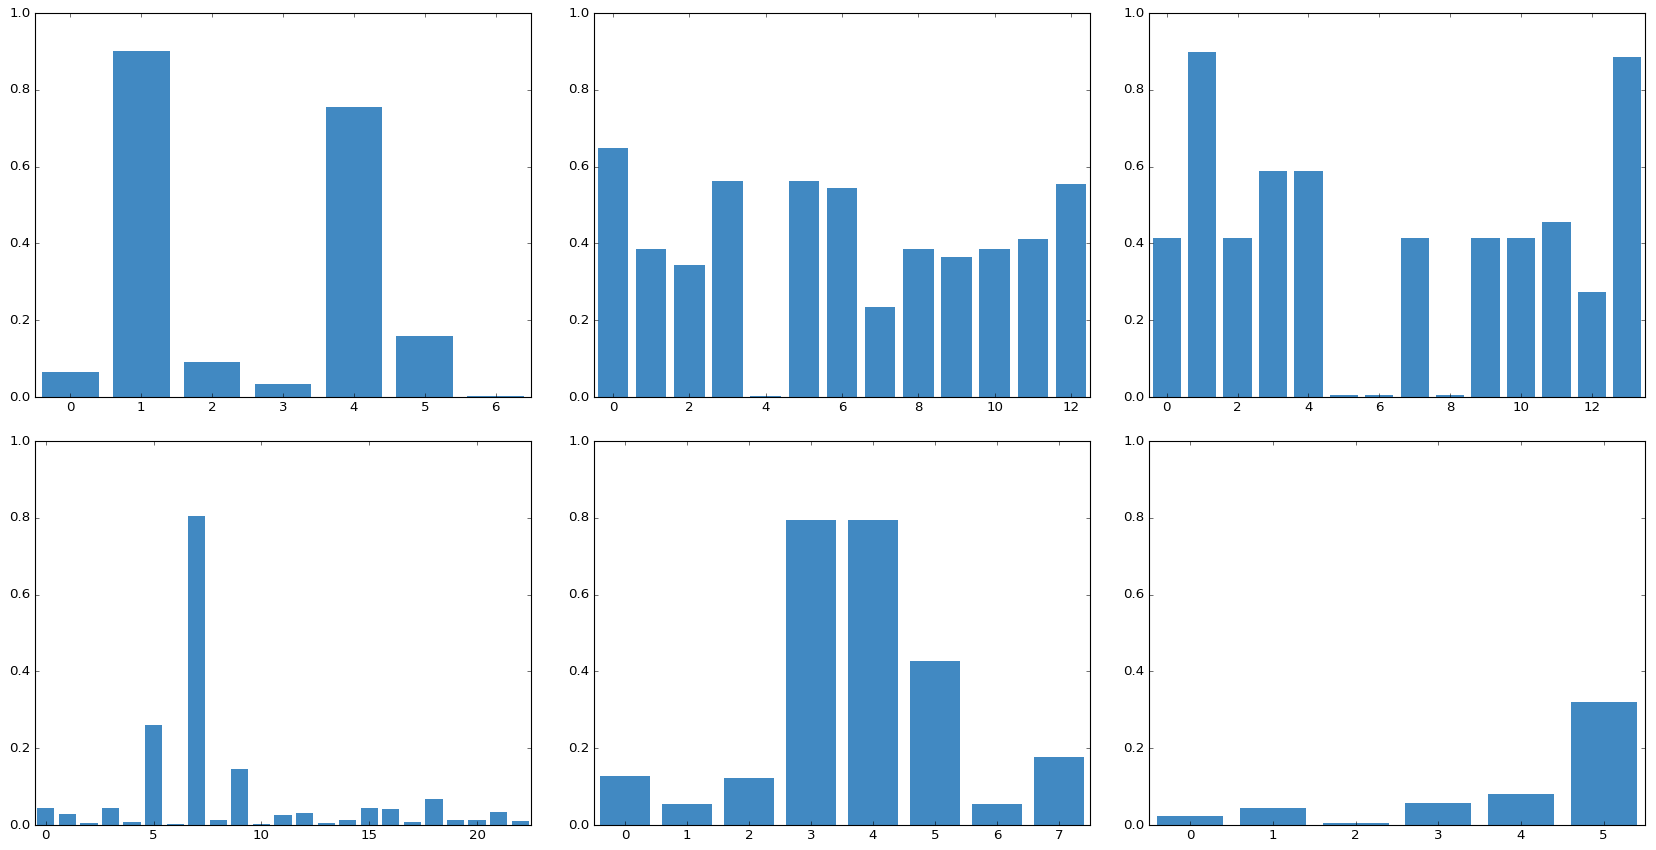
\includegraphics[width=\linewidth]{resources/candidate-similarity.png}
  \caption{Visualisation of the cosine similarity between the selected thumbnail and candidates for multiple videos.}
  \label{figure: thumbnail similarity}
\end{figure}


\subsection{Topic clustering using metadata}
\label{topic clustering}
% Data gathering and processing

% Selecting K
As described in section \ref{section: dataset requirements}, the videos in the dataset are not limited to a single domain and the selected thumbnails vary in contents throughout the whole dataset. In order to improve accuracy and provide a better prediction of positive video thumbnails, the dataset is clustered into specific topics using the metadata available.

Since specific topic categorisation is not available and the tags available in the metadata are not discriminative, a textual analysis of all metadata is used. The title, description and tags are concatenated and a stoplist is used to remove regular words. A bag-of-words corpus is formed with the resulting documents, which is used to create a latent Dirichlet allocation model with a number of topics $T = 25$. This value for $T$ is chosen because our domain only includes news related documents, while a value of 100 is reasonable for the whole Wikipedia dataset \cite{Newman:2009uk,Blei:2003tn}.

% Topic clustering using kmeans
With the LDA model, a sparse vector representation of the video metadata is generated which can be used to cluster the videos in the dataset. Clustering is done using K-means with $M$ clusters. A larger $M$ would mean more specific topics and more accurate SVM predictions, but will also reduce the number of samples for each topic. We found that the ideal value of M would be around 10, which results in a good balance between the number of samples per topic and inertia of the clusters. The scores of the SVM are visualised against different values for M in figure \ref{figure: svm accuracy with k}. An overview of the topic clustering can be found in figure \ref{figure: topic clustering scheme}.

\subsection{Model training}
\label{section: model training}
% Selecting videos based on topic

For each topic created in the topic clustering, an SVM is trained in order to rank new video thumbnail candidates. The data used for training an SVM consists of all the videos that are classified in that specific cluster (as described in section \ref{topic clustering}), along with the labels generated in section \ref{section: candidate evaluation}. In order to avoid overfitting the data, we use the same parameter $C = 10$ for each SVM, which resulted in an average accuracy of 0.79.

\begin{figure*}[tb!]
	\centering
	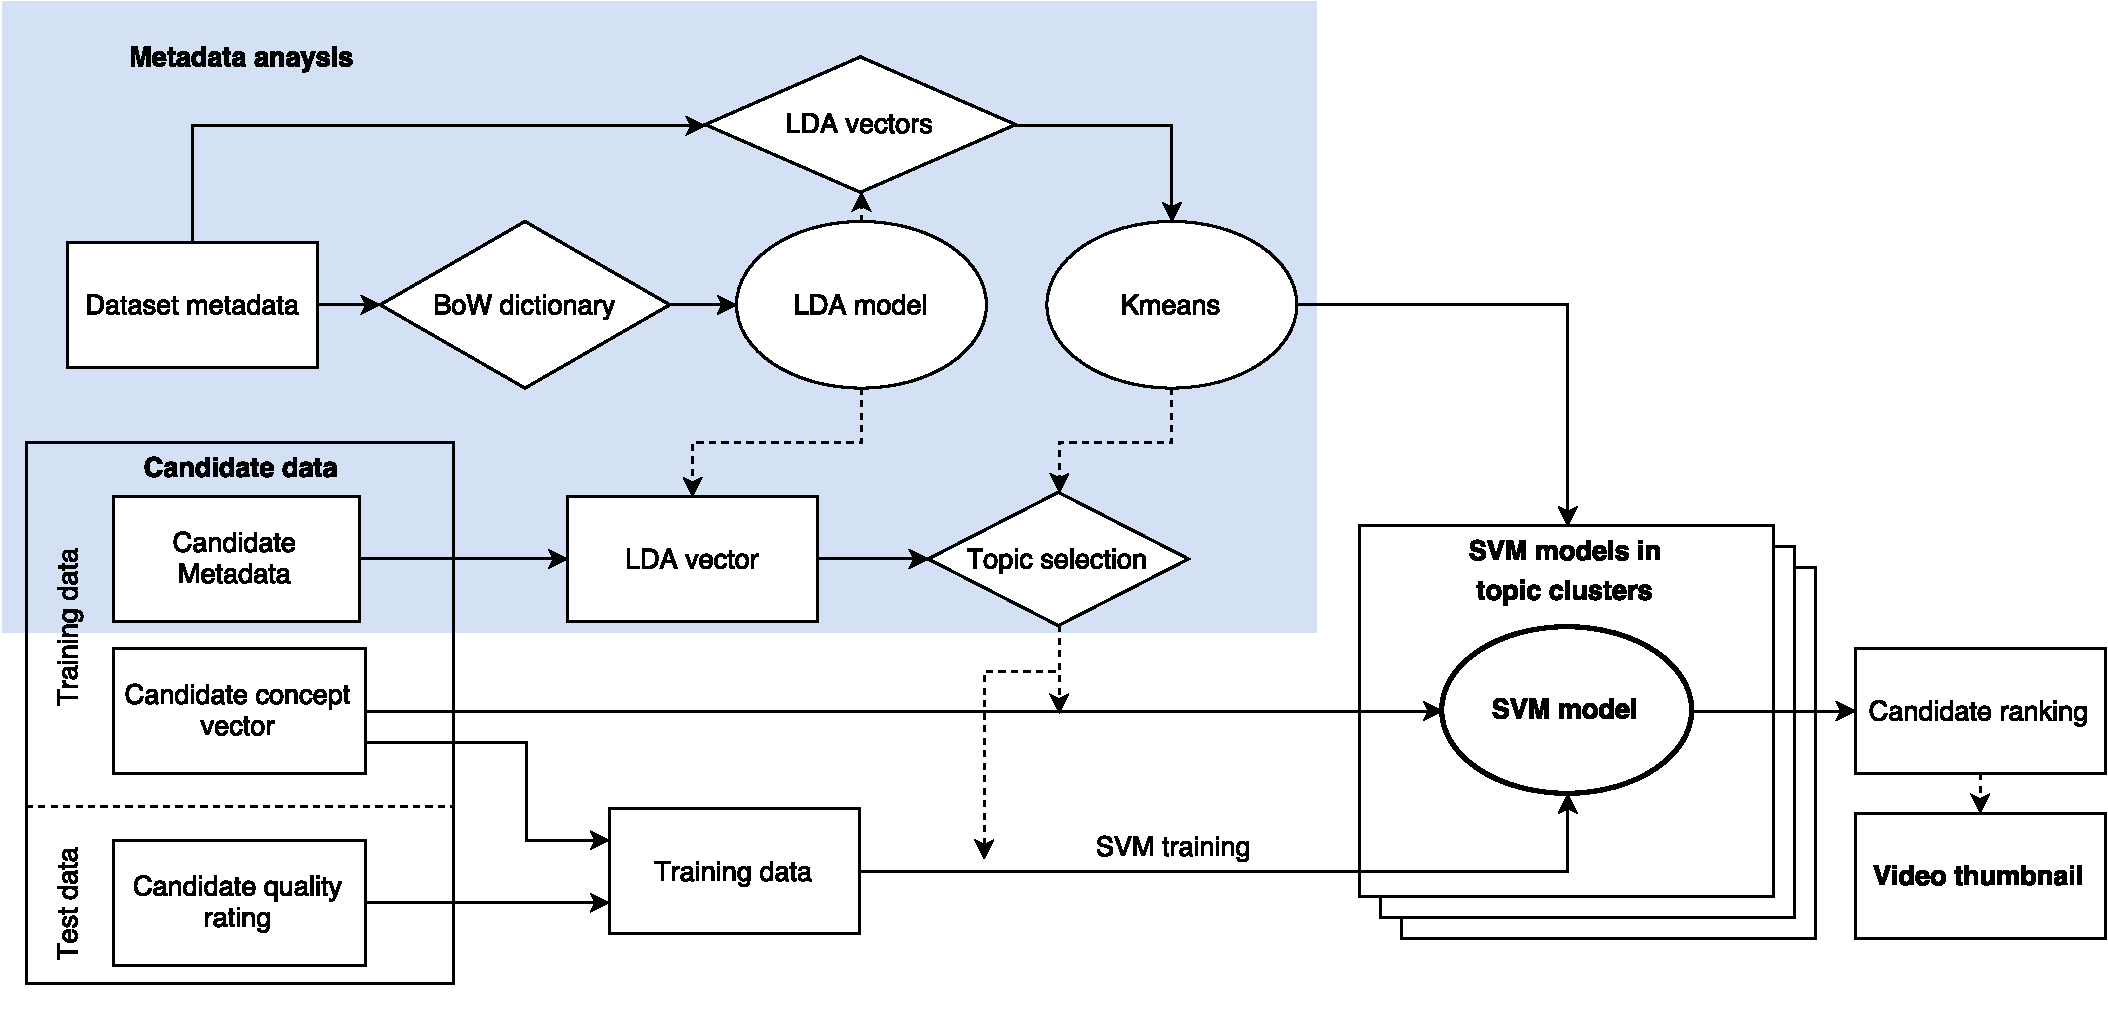
\includegraphics[width=0.9\textwidth]{resources/topic-clustering}
	\caption{Clustering videos in the dataset based on metadata using KMeans clustering on LDA topic vectors.}
	\label{figure: topic clustering scheme}
\end{figure*}

\subsection{Predicting new videos}

New videos with related textual metadata can be processed using our method to generate a video thumbnail. First, the frames are analysed with 1 fps to concept vectors as described in section \ref{section: feature extraction}. These frames are then used to create a list of candidates as described in section \ref{section: candidate selection}. The textual metadata is converted to a bag-of-words, which is then converted to an LDA vector with the model generated in \ref{topic clustering}. This vector can then be used to decide on the model to use. The concept vector representation of the video thumbnail candidates are then applied to the model (trained in section \ref{section: model training}), which classifies the vectors. The final ranking is based on the scores that are associated with the classification.


\begin{figure}[h]
	\centering
	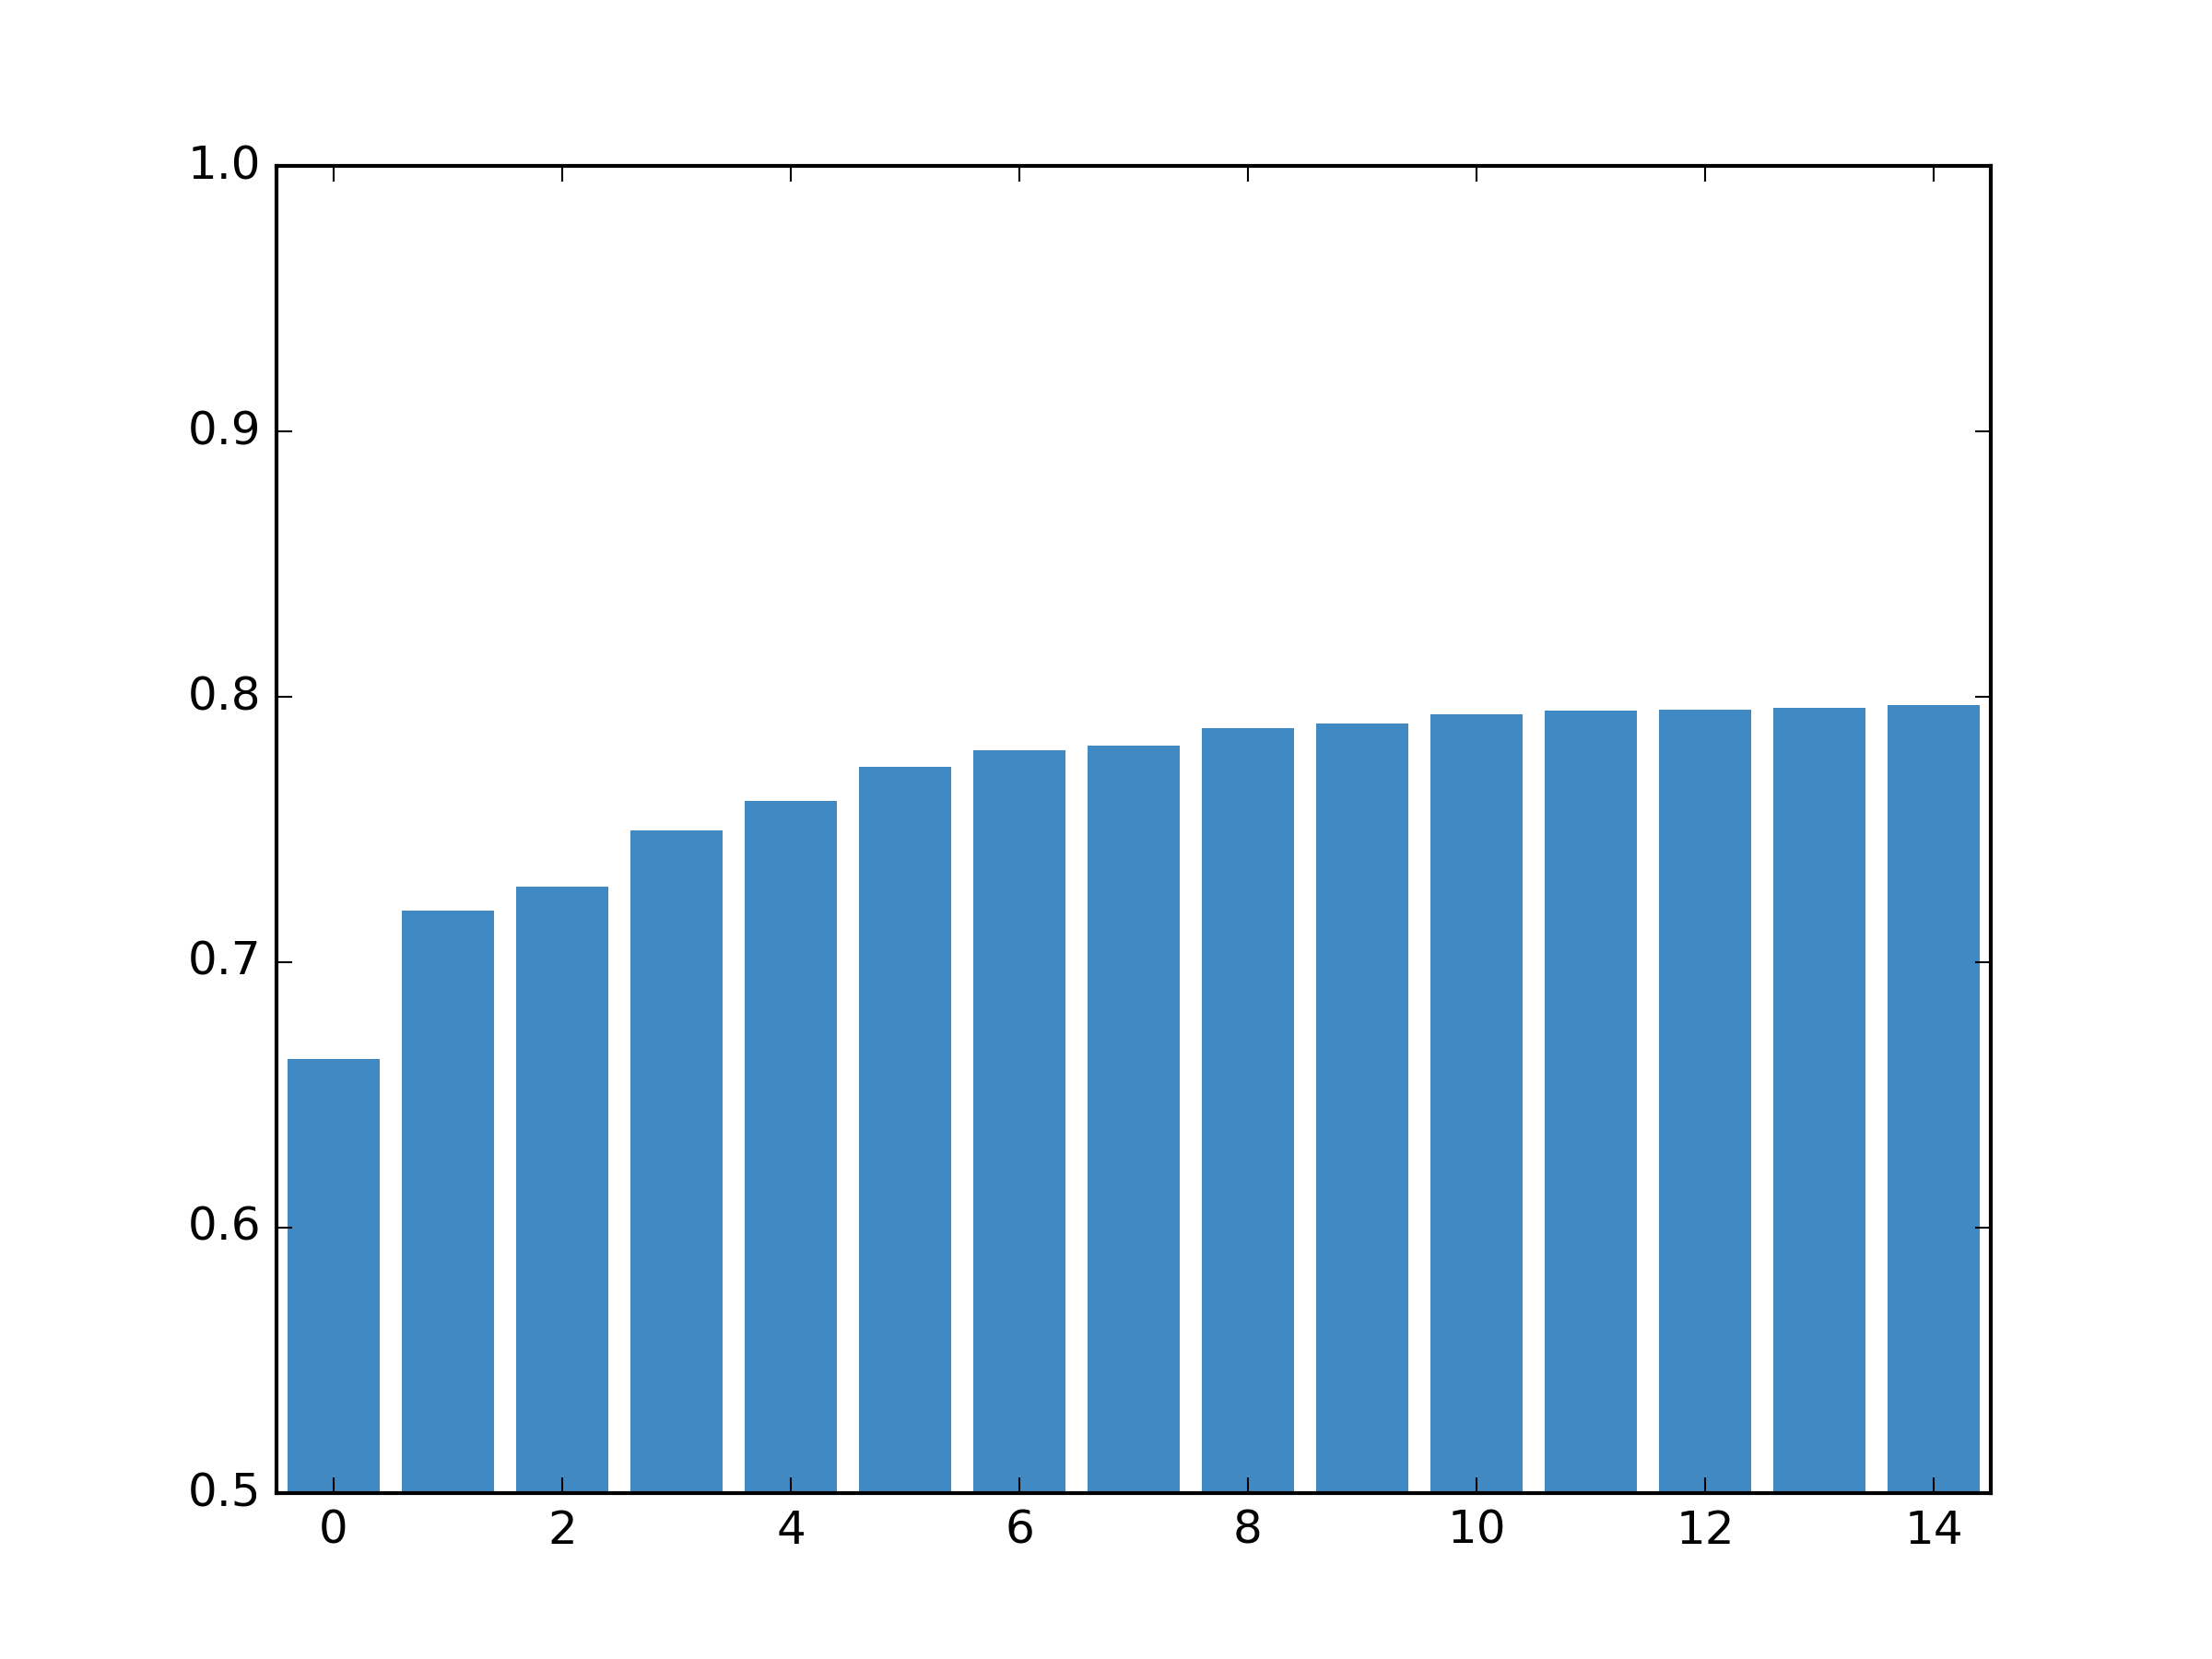
\includegraphics[width=\linewidth]{resources/svm-accuracy}
	\caption{SVM scores on different values of $M$ with a baseline of 0.5.}
	\label{figure: svm accuracy with k}
\end{figure}


\section{Experimental setup}
\label{experimental setup dataset}

The TRECVID Multimedia Event Detection track provides a number of datasets that can be used for event-detection training tasks, which are often used in video summarisation \cite{Ajmal:2012hi, Christel:2004in, Money:2008fn}. Other previous techniques in video highlighting and summarisation use data gathered from online platforms as YouTube and Facebook \cite{Yang:2015gi, Almeida:2012be}.

% Dataset source
The dataset that is used in our experimental setup is retrieved from the Irish online publisher `Landmark Digital' which is not publicly available. The news websites from this publisher publish news articles on a broad number of domains like world news, sports, business, life and local news. The videos are often published alongside an article that could be categorised in any domain. The dataset, however, does not contain any references to the related articles or domains.

% Dataset values
The videos in the dataset are accompanied by metadata in the form of a title, description and an unspecified number of (free-form) tags. This (editor created) metadata is primarily used for search engine optimisation and does not contain any structure other than the three values specified. Since these values are created by a professional news editor, we can assume that the data in these fields is a good representation of the content.

% Dataset thumbnail
As stated in section \ref{section: dataset requirements}, the approach requires thumbnails associated with the videos in the dataset to serve as positive examples for training purposes. All videos in our dataset contain a thumbnail, of which only a portion of these thumbnails is selected by an expert (in our case an editor for an online newspaper). The remaining thumbnails are automatically generated and cannot serve as reliable training examples, since an editor hasn't made a conscious decision about the contents in the thumbnail. This means that only a portion of our dataset can be used in the training stage of our system. These statistics can be viewed in table \ref{table:dataset}.

\begin{table}[h]
\caption{Overview of the dataset used in the experimental setup.}
\label{table:dataset}
\begin{tabular}{ll}
Total clips                    & 2162 \\ \hline
With title                     & 2162 \\
With description               & 1912 \\
With tags                      & 1690 \\
With selected thumbnail        & 956 
\end{tabular}
\end{table}


\section{User study}
\label{section: user study}

The video thumbnails generated by an implementation of the method described in section \ref{section: system description} have been tested in an A/B user survey against a baseline in the form of static thumbnails: 50\% of the respondents received the survey which included video thumbnails, while the other 50\% received a version with static thumbnails. The survey was conducted via a custom built website to ensure compatibility across multiple devices.

The user study is conducted to answer the following questions about the use of thumbnails in video previews:

\begin{itemize}
	\item \textbf{Q1.1} What is the effect of a thumbnail on the information received by the user?
	\item \textbf{Q1.2} What is the effect of a thumbnail on the engagement of the user?
	\item \textbf{Q2.1} What is the effect of a video thumbnail compared to a static thumbnail on the information received by the user?
	\item \textbf{Q2.2} What is the effect of a video thumbnail compared to a static thumbnail on the engagement of the user?
\end{itemize}

With the answers to Q1.1 and Q1.2, we can confirm that our survey aligns with our rationale based on related work on thumbnails described in \ref{section: video navigation}. We then can evaluate the answers to Q2.1 and Q2.2 and depict a conclusion on the effect of a video thumbnail in comparison to a static thumbnail.

\subsection{Hypothesis}

The following hypotheses can be formulated for the questions stated in section \ref{section: user study}:

\begin{itemize}
	\item \textbf{H1.1} The use of a thumbnail in a video preview increases the information received by the user.
\end{itemize}

Based on the related work in section \ref{section: video navigation}, a visual preview increases the accuracy of the user finding relevant content. Thus, we expect that the addition of the only visual element in our survey (either a video thumbnail or static thumbnail) has a positive effect on the information that a user receives from the thumbnail.

\begin{itemize}
	\item \textbf{H1.2} The use of a thumbnail in a video preview increases the engagement of a user.
\end{itemize}

Research on interfaces and websites for online news shows a high influence of images on the engagement of users, as described in section \ref{section: user engagement}. We expect that a similar influence is visible in our experiment by the introduction of any thumbnail.

\begin{itemize}
	\item \textbf{H2.1} The use of a video thumbnail increases the information received by the user compared to the use of a static thumbnail.
\end{itemize}

The addition of moving images to the thumbnail increases the amount of raw information displayed in the preview, so one could argue that the amount of information conveyed to the user is also increased. Related work discussed in section \ref{section: video navigation} also highlights an improvement of user accuracy in search results when comparing video summaries to a series of static video frames.

\begin{itemize}
	\item \textbf{H2.2} The use of a video thumbnail increases the engagement of a user compared to the use of a static thumbnail.
\end{itemize}

Based on the increased attention and interest towards certain items caused by visual elements as described in \ref{section: video navigation}, we hypothesise that the addition of motion in the thumbnail increases the interest of a user even further.

\subsection{Survey setup}
For each video, two previews were shown in successive order: The first preview contained only a title and description, while the second preview contained a title, description and a (static or video) thumbnail. An example of the preview with thumbnail is shown in figure \ref{figure: survey preview}.

\begin{figure}[h]
  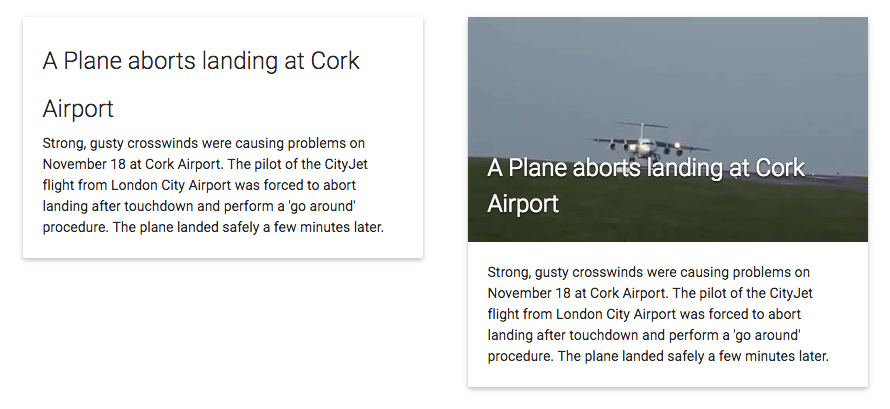
\includegraphics[width=\linewidth]{resources/preview-combined.png}
  \caption{An example of a video preview. A version without thumbnail is displayed on the left, while a version with thumbnail is displayed on the right.}
  \label{figure: survey preview}
\end{figure}

After each preview, two statements were made about the video preview to measure the engagement of the participant towards the video, and wether the participant felt informed about the contents of the video (we will refer to these statements as \textit(context):

\begin{itemize}
	\item I am interested in viewing the video (engagement).
	\item I know what to expect from the video (informative).
\end{itemize}

By comparing the difference in answers between the version with thumbnail and without thumbnail, we are able to measure the impact of using a thumbnail in the preview. This difference can then be compared between the static thumbnail and video thumbnail, allowing us to analyse the effect of a video thumbnail. This way, any preconception from the user about certain topics or videos can be taken into account.

The videos used in this survey were manually picked from the dataset based on number of views. Early feedback on the survey setup revealed that randomly selected videos would be uninteresting and yield no change in response, regardless of the form of the video preview. The difference in target audience between the dataset source and survey respondents would be the primary explanation. The age of most of the videos is a second explanation, since most of the news videos are outdated at the point of conducting the survey. Static thumbnails for the videos were picked at the time of publishing the original video, while the video thumbnails were generated using the method described in section \ref{section: system description}.

\subsection{Responses}

A total of 53 respondents participated, of which 27 received the version with video thumbnails, and 26 received the version with static thumbnails. Each participant received previews for a total of three videos, resulting in a total of 137 responses, of which 68 refer to the static thumbnail and 69 refer for the video thumbnail. An overview of these numbers can be found in table \ref{table: number of responses table}.

\begin{table}[h]
\centering
\begin{tabular}{@{}llll@{}}
\textbf{}             & \textbf{Total} & \textbf{Static} & \textbf{Video} \\ \toprule
\textbf{Participants} & 53             & 26              & 27             \\ \midrule
\textbf{Preview 1}    & 47             & 23              & 24             \\
\textbf{Preview 2}    & 46             & 23              & 23             \\
\textbf{Preview 3}    & 44             & 22              & 22             \\ \bottomrule
\textbf{Total}        & 137            & 68              & 69             \\
\end{tabular}
\caption{Response overview}
\label{table: number of responses table}
\end{table}

The difference between the expected number of responses ($53 * 3 = 159$) and the actual number of responses (137) can be explained by the fact that the participants could interrupt the survey at any time. Responses where the participant interrupted the survey between a preview without a thumbnail, and a preview with a thumbnail were ignored.

\subsection{Result analysis}

The data is gathered from two tests, one with static thumbnails and one with video thumbnails. The research questions are deliberately divided into two groups. In the first group of questions (Q1), we can test our survey setup with established work and further investigate the effect of the video thumbnail (Q2).


\subsubsection{Excluding thumbnail versus including thumbnail}
\label{section:excluding vs including}

Using the Wilcoxon signed-rank test for ordinal, paired data, a highly significant difference is found between previews including thumbnails and excluding thumbnails regarding information and engagement. The P-values are depicted in table \ref{table:significance}.

\begin{table}[h]
\centering
\begin{tabular}{@{}lll@{}}
                   & \textbf{P-value} \\ \hline
Information (Q1.1) & \num{1.00e-14}   \\
Engagement (Q1.2)  & \num{3.19e-10}
\end{tabular}
\caption{Significance of the difference between responses on previews with a thumbnail and without a thumbnail.}
\label{table:significance}
\end{table}

The responses reveal an overal increase in engagement when using thumbnails. These results align with the findings in other work described in \ref{section: video navigation}, and allow us to further investigate the differences between the static thumbnail and the video thumbnail in this topic in \ref{section: static versus video}. The responses are visualised in figure \ref{figure:information including excluding}.

\begin{figure}[h]
	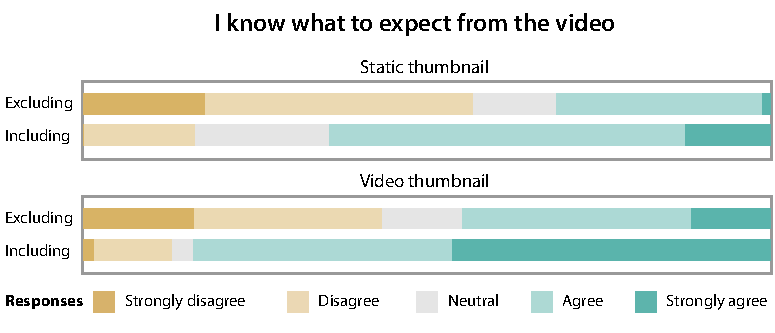
\includegraphics[width=\linewidth]{resources/information_including_excluding}
	\caption{Visualisation of the responses regarding \textbf{information} on static and video thumbnails, grouped by presence of the thumbnail.}
	\label{figure:information including excluding}
\end{figure}

The same Wilcoxon signed-rank test is used for the responses regarding engagement, where a highly significant difference is found. The same patterns that were found for information are visible, an overal increase is found when including thumbnails, though the change is more subtle. The responses are visualised in figure \ref{figure:engagement including excluding}.

\begin{figure}[h!]
	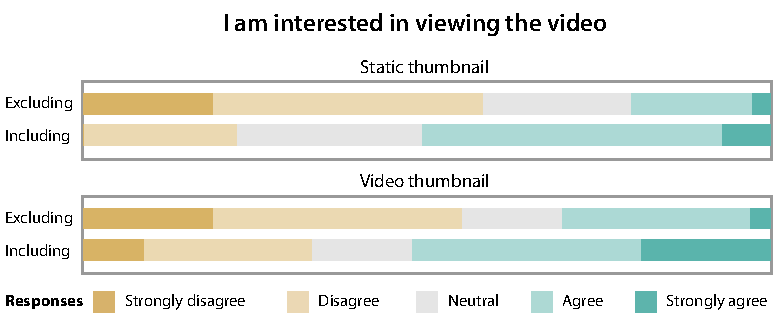
\includegraphics[width=\linewidth]{resources/engagement_including_excluding}
	\caption{Visualisation of the responses regarding \textbf{engagement} on static and video thumbnails, grouped by presence of the thumbnail.}
	\label{figure:engagement including excluding}
\end{figure}

\subsubsection{Static thumbnail versus video thumbnail}
\label{section: static versus video}

With the highly significant differences between static thumbnails and video thumbnails found in \ref{section:excluding vs including}, we can further investigate the differences between them. We use a Mann-Whitney U test on the ordinal data from these unpaired groups.

In order to analyse the responses in an objective manner, we need to compare the differences between the static group and video group for previews excluding a thumbnail. Since these previews were exactly the same among these two groups, we hypothesise that there is no significant difference between these groups.

\begin{table}[h]
\centering
\begin{tabular}{@{}llll@{}}
% 0.00065254
\textbf{P-value}   & \textbf{Including} & \textbf{Excluding} \\ \hline
Information (Q2.1) & 0.0006             & 0.0414             \\
Engagement (Q2.2)  & 0.7641             & 0.3935
\end{tabular}
\caption{Significance of the differences between static thumbnails versus video thumbnails, including and excluding the thumbnail.}
\label{table: q2 significance}
\end{table}

The results stated in table \ref{table: q2 significance} tell us a few things. First of all, there is \textbf{no significant difference} regarding engagement between the groups, including or excluding the thumbnail. Regarding information, a \textbf{highly significant difference} was found when a thumbnail was included, and a \textbf{significant difference} was found when the thumbnail was excluded.

While there is a highly significant difference between static thumbnails and video thumbnails regarding information, we cannot directly draw any conclusions, since a significant difference was also found between these groups when the thumbnail was absent. This means that the hypothesis stating that there is no significant difference between the two groups when excluding the thumbnail is rejected, and an in-depth analysis is required to gain any meaningful insights about the effects of the video thumbnail.

Since the Likert responses are categorised as ordinal data, we cannot calculate the differences or mean values between these groups. Instead, the responses are categorised into five different groups by the response on the preview without a thumbnail. This way, we can analyse the effect of a thumbnail while any initial response on a topic is taken into account. A detailed visualisation of this data is shown in \ref{figure:information static versus video}, while the uncategorised responses are shown in figure \ref{figure:information including excluding} (static thumbnail: including - video thumbnail: including).

\begin{figure}[h]
	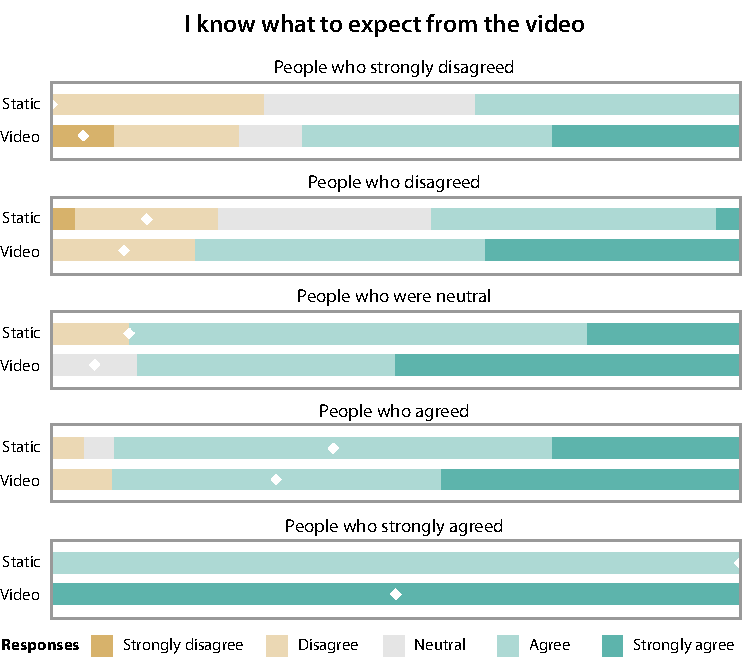
\includegraphics[width=\linewidth]{resources/information_static_video}
	\caption{Effect of static thumbnails versus video thumbnails, regarding information, categorised by response on the preview without a thumbnail. Responses that align with the initial response are marked with a white indicator to highlight the baseline for each category.}
	\label{figure:information static versus video}
\end{figure}

In the `strongly disagree' category, more than half of the respondents shifted to a positive answer when they received a preview with video thumbnail. The same shift is also visible in the `disagree' category, both categories show a reduction in the amount of negative responses. Looking at the neutral and positive responses, a clear contrast is apparent in the amount of `neutral' and `strongly agree' responses. This increase shows that the positive effect of a thumbnail is amplified with the use of a video variant.

In the `neutral' category, a positive change in response is clearly visible in both static and video thumbnails. Again, we see the amplified positive effect in the `strongly agree' responses for video thumbnails. The `agree' category shows a similar trend, although the the overall positive change is less noticeable. The number of responses in the category `people who strongly agreed' is too limited to draw any conclusions (both thumbnail variants contained only a single response for `strongly agree'), but is included in the visualisation for the sake of completeness.

\begin{figure*}[tb!]
	\centering
	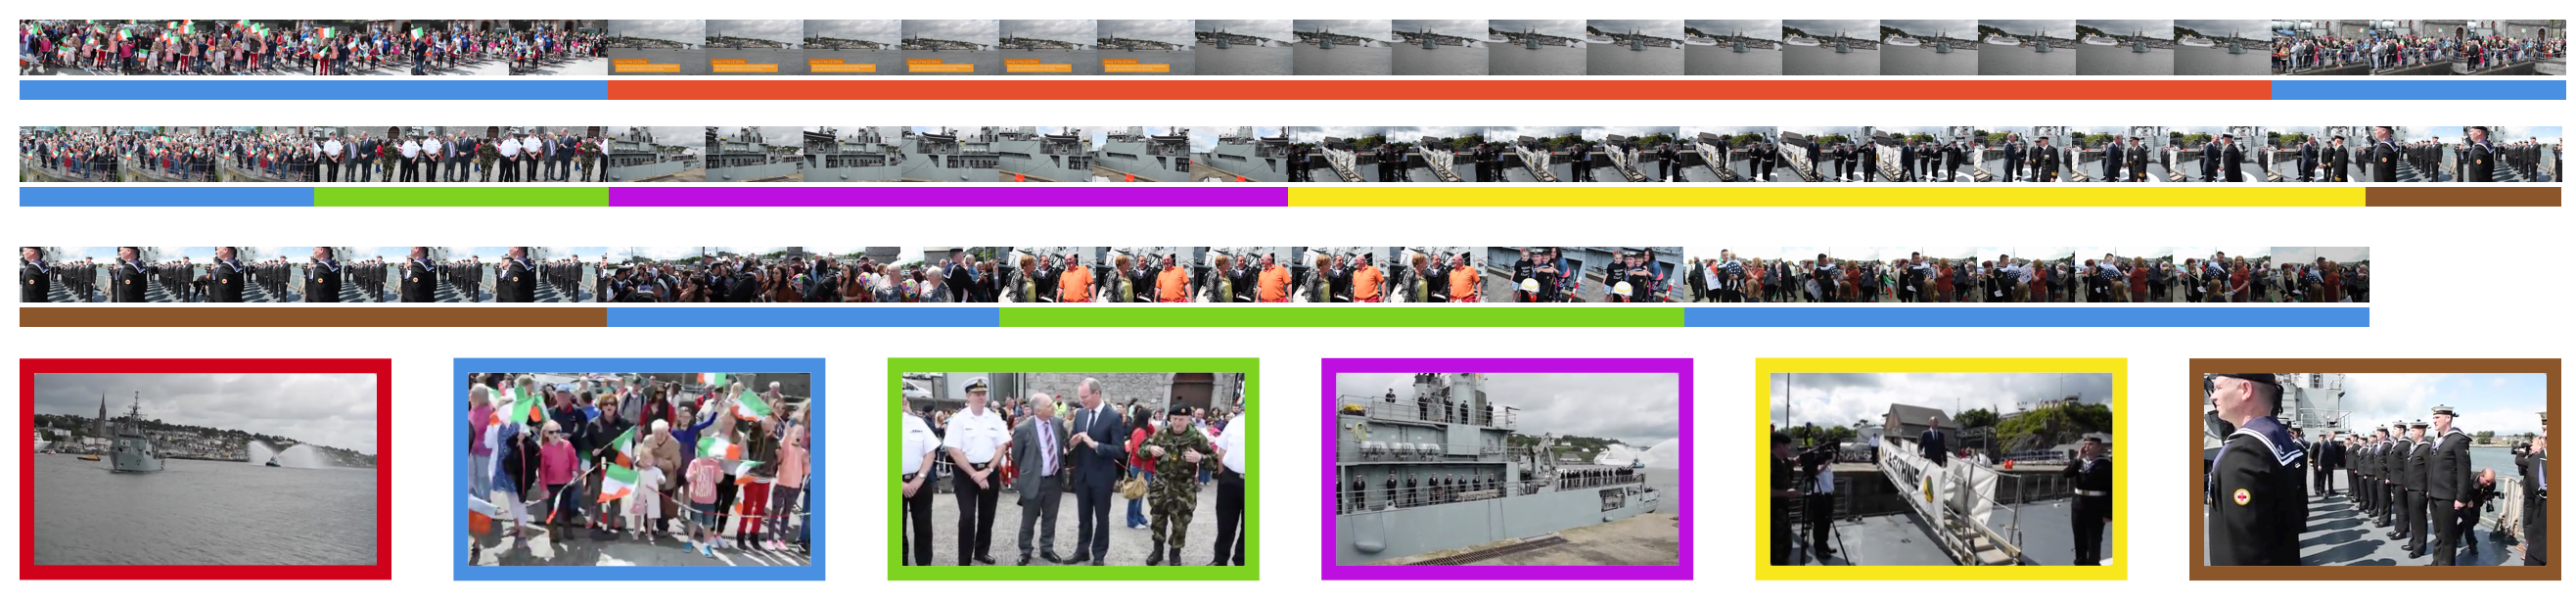
\includegraphics[width=\textwidth]{resources/clustering.png}
	\caption{An example of the bag of fragment clustering. The coloured bars on the top indicate what frames are placed in which cluster. The frames below are the selected candidates from each topic.}
	\label{figure: topic clustering example}
\end{figure*}

We can conclude that the use of a video thumbnail amplifies the positive effect caused by the use of a thumbnail in regard to the information that a user obtains from a video preview. While our responses show a hint of the same effect on the engagement (figure \ref{figure:engagement including excluding}, we are unable to draw any conclusions since they are not significantly different. With an in-depth study containing more controlled variables, a larger sample size and a real-world environment, a better understanding of the effect on engagement can be developed.

\section{Conclusion}

In this paper, we conclude that it is possible to automatically generate video thumbnails that have a positive effect on users compared to static thumbnails which are commonly used today. Based on the results from our user study, we conclude that the implementation of the techniques from the field of video summarisation play a crucial part in the improved information that users experienced. We believe that our method of candidate selection results in a conceptually diverse set candidates, which play an important role in the improvement of information.

User engagement is a highly complex topic where many variables are at play in complex situations. Although our results do not directly show a significant difference between video thumbnails and static thumbnails, we have reasons to believe that the video thumbnail will affect user engagement when an approach is used that better fits the specific intent and purpose of the video thumbnail. Our method of extracting video thumbnails is largely based on techniques used in video summarisation, where the primary concern is to extract information instead of improving user engagement. Using a thumbnail selected by an expert as evaluation data is a step in the right direction, and we suggest that alterations like these to video summary techniques will greatly improve the engagement of the video thumbnails.

New interfaces that facilitate video thumbnail selection for editors will allow us to further analyse the choices made for specific video thumbnails, which could lead to new insights and allow us to adjust our methods of selection and evaluation. The effects of large scale, real-world implementations of video thumbnails could also be utilised to gain new insights in the behaviour of users with this new interface element. Finally, we conclude that the promising effects of video thumbnails should be utilised in the application of previews for videos in order to improve user experience.
 
\section{Acknowledgements}

Special thanks to Jan Zahálka for the exceptional supervision on this master thesis. His insights and knowledge in the field of multimedia analysis provided crucial leads to various techniques and methods that were used. We would also like to thank the people at Landmark Digital, who provided us with the initial idea of video thumbnails and allowed us to use their data for experimentation. Finally, the people at Blue Billywig are thanked for their support and general knowledge regarding (online) video.
%
%
%From the results from the user study give us valuable information about the way video thumbnails affect users. The effects of static thumbnails are a well researched topic, where the general consensus is that a visual preview increases the user experience. Our study shows that, regarding the engagement and information towards the user, the video thumbnail is not different than the static thumbnail. An important finding in our study, is that the video thumbnail does not perform worse than the static alternative, thus can safely be used as an alternative. This poses new possibilities in interface design and user experience design, where media interfaces can be enhanced with moving images.
%
%Further testing the video thumbnail is an important next step in the evolution of this new interface element. We expect that a moving thumbnail can improve the visual attractiveness of an interface, when implemented in a correct way. The video thumbnail may sparsely be used in an interface that uses static thumbnails to focus the attention of the user to a specific videos. The effect of the video thumbnail on these topics can be tested in a practical scenario, but are hard to objectively test in an isolated survey.
%
%The system that we designed and described in section \ref{section: system description} contains much of the techniques from video summarisation. We believe that a system that automatically generates video thumbnails can much be improved by implementing techniques created specifically for the tast of video thumbnail generation. A big first step in the improvements would be the creation of a benchmark dataset, which can be used to train and test new systems. A repetition of the user study described in section \ref{section: user study} using generated video thumbnails from improved system might show a significant difference.

\printbibliography

\balancecolumns

\end{document}







